
\documentclass[12pt,a4paper]{article}

% Configuración del documento
\usepackage[spanish,es-nodecimaldot]{babel}
\usepackage[utf8]{inputenc}
\usepackage[T1]{fontenc}
\usepackage{lmodern}
\usepackage{geometry}
\usepackage{setspace}
\usepackage{graphicx}
\usepackage{float}
\usepackage{booktabs}
\usepackage{longtable}
\usepackage{array}
\usepackage{enumitem}
\usepackage{csquotes}
\usepackage{hyperref}


\geometry{
    left=2.5cm,
    right=2.5cm,
    top=2.5cm,
    bottom=2.5cm
}

\onehalfspacing


\usepackage[
    backend=biber,
    style=ieee,
    sorting=none
]{biblatex}

\addbibresource{referencias/jordan.bib}
\addbibresource{referencias/washington.bib}


\title{Sistema de Registro de Eventos Interculturales (SREI)}
\author{Proyecto Fin de Curso}
\date{Noviembre de 2026}

\begin{document}

\maketitle

\begin{center}
    \textbf{Aplicaciones Distribuidas}\\
    Universidad Técnica Estatal de Quevedo\\
    Periodo académico 2026--2027
\end{center}

\tableofcontents
\newpage


\section{Contexto y problema}

\subsection{Resumen ejecutivo}

El Sistema de Registro de Eventos Interculturales (SREI) es un proyecto que busca facilitar la organización y gestión de los eventos interculturales de la Universidad Técnica Estatal de Quevedo (UTEQ). La propuesta surge de la necesidad de contar con un espacio donde se pueda manejar de forma ordenada la información de los eventos, desde que un docente presenta una propuesta hasta que se realiza la actividad y se registra la participación de los asistentes.

Para conocer mejor esta situación, se realizó un levantamiento de información mediante entrevistas semiestructuradas a cuatro personas relacionadas con este proceso: la coordinadora de la carrera de Software, el decano de la Facultad de Ciencias de la Computación, una docente de la Facultad de Ciencias de la Educación con experiencia en la gestión de eventos y un estudiante de la carrera de Software. Cada participante aportó una perspectiva diferente sobre la forma en que deberían organizarse y gestionarse estas actividades.

Entre las necesidades identificadas se encuentran el envío digital de propuestas, la revisión y aprobación de solicitudes, la consulta de su estado y la administración de la información de los eventos. También se planteó la importancia de facilitar la inscripción de los participantes, confirmar su asistencia y disponer de información estadística sobre las actividades realizadas.

A partir de estos resultados, se propone desarrollar una aplicación web que reúna estas funciones y permita organizar sus responsabilidades mediante servicios independientes. La distribución de los componentes busca facilitar el mantenimiento y la evolución del sistema, además de permitir que sus diferentes partes puedan desarrollarse y desplegarse de manera organizada.

Durante el periodo académico se trabajará progresivamente en la construcción de esta solución. La primera etapa establece el problema, los objetivos, los requisitos y la arquitectura inicial. En las siguientes entregas se desarrollarán los servicios, la comunicación entre ellos, el manejo de datos y las pruebas necesarias para comprobar su funcionamiento.

De esta manera, el SREI pretende ofrecer una herramienta que responda a las necesidades identificadas durante las entrevistas y que facilite tanto el trabajo de quienes organizan los eventos como la participación de estudiantes y personas externas a la universidad.

\subsection{Antecedentes y contexto institucional}

El proyecto SREI se plantea para la Universidad Técnica Estatal de Quevedo, en el contexto de la organización y participación en eventos interculturales. En estas actividades intervienen diferentes personas, desde las autoridades y responsables de coordinación hasta los docentes que organizan los eventos y los estudiantes que participan en ellos.

Para conocer las necesidades de estos grupos, se realizó un levantamiento de información mediante cuatro entrevistas semiestructuradas. Los participantes fueron la coordinadora de la carrera de Software, el decano de la Facultad de Ciencias de la Computación, una docente de la Facultad de Ciencias de la Educación que cuenta con experiencia en la gestión de eventos dentro de esa facultad y un estudiante de la carrera de Software.

Las entrevistas permitieron conocer distintas necesidades según las responsabilidades de cada participante. Mientras que las autoridades y la coordinación se enfocaron principalmente en la revisión, administración y supervisión de los eventos, la docente aportó desde su experiencia en la organización de estas actividades. Por su parte, el estudiante permitió conocer las necesidades de quienes participan en los eventos.

\subsection{Descripción del problema}

La organización de un evento intercultural requiere coordinar varias actividades. Primero se debe presentar una propuesta, después revisarla y aprobarla, preparar su difusión y, finalmente, facilitar la participación de las personas interesadas. En este proceso intervienen distintos responsables, por lo que es importante mantener la información organizada y permitir que cada uno conozca el estado de las actividades que tiene a su cargo.

Durante las entrevistas se identificó la necesidad de facilitar el envío digital de propuestas, consultar el estado de las solicitudes y gestionar la información de los eventos. También se señalaron aspectos relacionados con la inscripción de participantes, la confirmación de asistencia y la consulta de estadísticas después de realizar las actividades.

Estas necesidades muestran que hace falta una herramienta que reúna la información y facilite el seguimiento de las distintas etapas de gestión. Por ello, el problema que busca atender el SREI es la falta de un mecanismo centralizado que permita organizar estos procesos y mantener una comunicación más clara entre quienes proponen, administran y participan en los eventos.

El informe de entrevistas no contiene mediciones cuantitativas sobre los tiempos empleados, los costos o la cantidad de errores del procedimiento actual. Por esta razón, no se presentan cifras como resultados comprobados; estos datos deberán obtenerse mediante mediciones adicionales si se requiere establecer una línea base.

\subsection{Identificación de los interesados}

A partir de las entrevistas realizadas se identificaron cuatro perfiles principales que tienen relación directa con el funcionamiento del sistema:

\begin{itemize}

    \item \textbf{Coordinación de la carrera de Software:} necesita recibir las propuestas de eventos, revisarlas y aprobarlas o rechazarlas. También requiere gestionar la información de los eventos y consultar estadísticas que permitan conocer los resultados de las actividades realizadas.

    \item \textbf{Decanato de la Facultad de Ciencias de la Computación:} necesita supervisar la gestión de los eventos, controlar la asignación de usuarios con privilegios administrativos y disponer de informes estadísticos sobre las actividades desarrolladas.

    \item \textbf{Docentes organizadores de eventos:} necesitan enviar sus propuestas de manera digital, incluir la información correspondiente y consultar el estado de las solicitudes para conocer cómo avanza su revisión. También manifestaron interés en contar con herramientas de apoyo para la creación de contenido visual.

    \item \textbf{Estudiantes de la carrera de Software y usuarios externos:} necesitan consultar los eventos disponibles, registrarse para participar y confirmar su asistencia a las actividades programadas.

\end{itemize}


\subsection{Objetivos del proyecto}

\subsubsection{Objetivo general}

Desarrollar un sistema web distribuido para apoyar la gestión de eventos interculturales de la Universidad Técnica Estatal de Quevedo, facilitando el registro de propuestas, su revisión y aprobación, la administración de eventos y la participación de estudiantes y usuarios externos.

\subsubsection{Objetivos específicos}

\begin{enumerate}

    \item \textbf{Identificar y documentar las necesidades de los interesados} mediante el análisis de las entrevistas y la revisión de los requisitos existentes, para establecer las funcionalidades que debe cubrir el sistema.

    \textit{Indicador:} Porcentaje de requisitos identificados que cuentan con una fuente documentada y trazabilidad.

    \item \textbf{Diseñar una arquitectura distribuida} que permita separar las principales responsabilidades del sistema y establecer mecanismos de comunicación entre sus servicios.

    \textit{Indicador:} Número de servicios definidos e integrados de acuerdo con la arquitectura propuesta.

    \item \textbf{Implementar las funcionalidades principales del sistema} para gestionar propuestas, eventos, usuarios e inscripciones, de acuerdo con los requisitos establecidos.

    \textit{Indicador:} Porcentaje de funcionalidades implementadas que superan sus respectivas pruebas de aceptación.

    \item \textbf{Verificar el funcionamiento y la calidad de la solución} mediante pruebas de integración y evaluación de los requisitos funcionales y no funcionales.

    \textit{Indicador:} Porcentaje de casos de prueba ejecutados satisfactoriamente respecto del total de casos definidos.

\end{enumerate}


\subsection{Trabajos relacionados}

Para el desarrollo del SREI se revisaron investigaciones relacionadas con la administración de eventos y el uso de aplicaciones web en contextos culturales y universitarios. Estos trabajos permiten conocer algunas soluciones que ya se han desarrollado y tomar como referencia sus funcionalidades y enfoques de implementación.

Ogbiti y Jumai (2024) presentan un sistema web para la gestión de eventos que permite realizar actividades como la creación de eventos, el registro de participantes y el envío de notificaciones. La propuesta utiliza tecnologías web y una base de datos para facilitar la administración de las actividades. En las pruebas realizadas con datos de muestra, los autores reportan que el sistema permitió gestionar eventos y registros de participantes, además de proporcionar actualizaciones en tiempo real. Este trabajo resulta de interés para el SREI porque aborda funciones relacionadas con la organización y participación en eventos. Sin embargo, el proyecto que se desarrolla para la UTEQ también contempla la gestión de propuestas y su revisión dentro del entorno institucional \cite{ogbiti2024}.

Por otra parte, Chaturvedi et al. (2024) desarrollan CU-EVENTS, una plataforma orientada a la gestión de eventos universitarios. El sistema reúne funcionalidades como el registro de usuarios, la publicación de eventos, la inscripción de estudiantes, el seguimiento de asistencia mediante códigos QR y la generación de certificados de participación. Además, propone una arquitectura de tres capas que separa la presentación, la lógica de aplicación y la base de datos. Esta investigación aporta una referencia importante para el SREI, especialmente en la organización de usuarios y el seguimiento de la participación estudiantil. La diferencia principal está en que SREI también busca atender las necesidades de presentación y revisión de propuestas de eventos interculturales en la universidad \cite{chaturvedi2024}.

En el contexto ecuatoriano, Argudo-Piedra y Sañay-Sañay (2025) presentan una aplicación web para la administración y coordinación de eventos culturales en la Casa Cultural de Cuenca. La solución permite centralizar actividades como la gestión de usuarios, las reservas de salas, el control de inventarios y la programación de eventos mediante un calendario interactivo. Para su desarrollo se utilizaron el marco AUP y el modelo de calidad FURPS+, además de tecnologías como React, Node.js y Express. Los resultados descritos muestran que la aplicación permitió organizar estos procesos desde una misma plataforma y facilitar la administración de las actividades culturales. Este trabajo tiene una relación cercana con el SREI por su orientación hacia la gestión cultural en Ecuador. No obstante, ambos proyectos responden a contextos diferentes, ya que el SREI está dirigido a la organización de eventos interculturales dentro de una institución universitaria \cite{argudo2025}.

A partir de la revisión de estas investigaciones se observa que existen propuestas que facilitan la creación de eventos, el registro de participantes, la difusión de actividades y la administración de información. También se identifican diferentes formas de organizar sus componentes, desde aplicaciones web con bases de datos hasta arquitecturas estructuradas por capas.

Estos aportes sirven como referencia para el desarrollo del SREI. Sin embargo, el proyecto plantea atender un contexto institucional específico, en el que también es necesario considerar la presentación de propuestas, su revisión y aprobación, la administración de los eventos y el registro de la participación. Por esta razón, se busca integrar estas necesidades en una solución web distribuida, tomando en cuenta los resultados del levantamiento realizado con los interesados de la UTEQ.


\section{Requisitos del sistema}

\subsection{Introducción}

En esta sección se presentan los requisitos del Sistema de Registro de Eventos Interculturales (SREI). Su definición parte de las necesidades identificadas durante el levantamiento de información y de la especificación de los módulos de Gestión de Usuarios y Roles y Propuesta del Evento.

Para organizar los requisitos se consideran las categorías de negocio (BRS), interesados (StRS), sistema (SyRS), calidad (QR) y restricciones (C), siguiendo la estructura de la norma ISO/IEC/IEEE 29148:2018.

\subsection{Fuentes y técnica de elicitación}

La entrevista semiestructurada fue la técnica utilizada para conocer las necesidades de las personas relacionadas con la organización y participación en eventos interculturales. Permitió orientar las preguntas según el perfil de cada interesado y profundizar en los aspectos que requerían mayor explicación.

Como fuentes documentales se consideran el informe de entrevistas del proyecto y las especificaciones de requisitos de Gestión de Usuarios y Roles y Propuesta del Evento. También se dispone de grabaciones de audio correspondientes a entrevistas y validaciones. Estas grabaciones se conservan como evidencias; no se presentan como transcripciones.

La información recopilada se organizó de acuerdo con las necesidades de los interesados y se relacionó con los requisitos correspondientes. Los identificadores de las especificaciones originales se mantienen para facilitar su seguimiento.

\subsection{Perfiles de los interesados}

Los perfiles que participan en la definición y validación de los requisitos se presentan a continuación.

\begin{longtable}{p{0.29\textwidth} p{0.63\textwidth}}
\caption{Perfiles de los interesados del SREI}\\
\toprule
\textbf{Interesado} & \textbf{Rol y responsabilidad}\\
\midrule
\endfirsthead
\toprule
\textbf{Interesado} & \textbf{Rol y responsabilidad}\\
\midrule
\endhead
Ing. Jéssica Alexandra Ponce Ordoñez &
Product Owner. Coordinadora de la carrera de Software de la FCCDD, UTEQ. Proporciona requisitos.\\
Ing. Washington Alberto Chiriboga Casanova &
Product Owner. Decano de la Facultad de Ciencias de la Computación y Diseño Digital, UTEQ. Proporciona requisitos.\\
Msc. Elizabeth Johanna Contreras Jara &
Product Owner. Docente de Educación Inicial de la Facultad de Ciencias de la Educación, UTEQ. Proporciona requisitos.\\
Dr. Gleiston Cicerón Guerrero Ulloa &
Scrum Master. Facilitador externo y tutor académico del proceso Scrum.\\
Washington Germán Apunte Pazmiño &
Integrante del equipo de desarrollo.\\
Jordan Josue Loor Suárez &
Integrante del equipo de desarrollo.\\
Steffanny del Rocío Loor Suárez &
Integrante del equipo de desarrollo.\\
Estudiante participante &
Usuario final que consulta los eventos, se registra y confirma su asistencia.\\
\bottomrule
\end{longtable}

\subsection{Clasificación de los requisitos}

Los requisitos se organizan en cinco grupos:

\begin{itemize}
    \item \textbf{BRS:} requisitos de negocio que expresan los objetivos institucionales.
    \item \textbf{StRS:} necesidades y expectativas de los interesados.
    \item \textbf{SyRS:} requisitos funcionales que describen las operaciones que debe realizar el sistema.
    \item \textbf{QR:} requisitos relacionados con la calidad, como usabilidad, rendimiento, seguridad y compatibilidad.
    \item \textbf{C:} restricciones que delimitan las tecnologías, formatos y condiciones de funcionamiento.
\end{itemize}

\subsection{Requisitos de negocio}

La especificación contempla dos requisitos de negocio principales:

\begin{itemize}
    \item \textbf{BRS-01:} controlar de forma centralizada el acceso al módulo y las acciones permitidas según el rol de cada persona.
    \item \textbf{BRS-02:} formalizar las propuestas de eventos interculturales, de manera que los eventos publicados cuenten con un informe PDF de respaldo y un trámite verificable.
\end{itemize}

\subsection{Requisitos de los interesados}

Se identifican las siguientes necesidades:

\begin{itemize}
    \item \textbf{StRS-01:} el Administrador necesita crear, consultar, actualizar y dar de baja a los usuarios.
    \item \textbf{StRS-02:} el Administrador necesita definir los roles y sus respectivos permisos.
    \item \textbf{StRS-03:} el Docente necesita registrar una propuesta de evento, adjuntar el informe PDF y enviarla a revisión.
    \item \textbf{StRS-04:} el Docente necesita registrar los campos particulares de cada tipo de evento, sin tener que utilizar campos genéricos.
\end{itemize}

\subsection{Historias de usuario}

A partir de los requisitos funcionales especificados para los módulos de Gestión de Usuarios y Roles y Propuesta del Evento, se presentan diez historias de usuario. Cada una incluye criterios de aceptación, prioridad y trazabilidad hacia los requisitos originales.

\begin{longtable}{p{0.07\textwidth} p{0.33\textwidth} p{0.36\textwidth} p{0.09\textwidth} p{0.11\textwidth}}
\caption{Historias de usuario y criterios de aceptación}\\
\toprule
\textbf{ID} & \textbf{Historia de usuario} & \textbf{Criterios de aceptación} & \textbf{Prioridad} & \textbf{Trazabilidad}\\
\midrule
\endfirsthead
\toprule
\textbf{ID} & \textbf{Historia de usuario} & \textbf{Criterios de aceptación} & \textbf{Prioridad} & \textbf{Trazabilidad}\\
\midrule
\endhead

HU-01 &
Como Administrador, quiero registrar usuarios con sus datos personales y correo institucional para mantener organizada la información de las personas que utilizan el sistema. &
El sistema solicita cédula, nombres, apellidos, correo institucional, contraseña y rol. El correo debe pertenecer al dominio @uteq.edu.ec. La cédula debe contener diez dígitos numéricos. &
Alta &
RF-01, RF-02, RF-03\\

HU-02 &
Como Administrador, quiero evitar registros duplicados para mantener información única de cada usuario. &
El sistema verifica que la cédula y el correo no estén registrados previamente. Si alguno está duplicado, rechaza el registro e informa el motivo. &
Alta &
RF-04\\

HU-03 &
Como Administrador, quiero modificar y desactivar usuarios para mantener actualizada la información y controlar quién puede acceder al sistema. &
El sistema permite modificar los datos del usuario y cambiar su estado. La desactivación conserva el registro y su historial de acciones. &
Alta &
RF-06, RF-07\\

HU-04 &
Como Administrador, quiero consultar y filtrar los usuarios registrados para encontrar rápidamente una cuenta. &
El listado permite filtrar por rol, estado, nombre, apellido o cédula. &
Media &
RF-08\\

HU-05 &
Como Administrador, quiero administrar los roles y permisos para controlar las acciones que puede realizar cada tipo de usuario. &
El sistema permite crear, consultar, modificar y eliminar roles y permisos. También permite asignar y revocar permisos, sin duplicar asignaciones. &
Alta &
RF-09, RF-10, RF-11, RF-12, RF-13, RF-14\\

HU-06 &
Como Docente, quiero registrar una propuesta de evento con sus datos principales para enviarla a revisión. &
El formulario solicita lugar, tipo de evento, título, descripción, fecha, hora de inicio y hora de fin. La hora de finalización debe ser posterior a la de inicio. &
Alta &
RF-17, RF-18, RF-19, RF-20, RF-21\\

HU-07 &
Como Docente, quiero adjuntar una imagen al evento y declarar su origen para identificar si fue cargada manualmente o generada mediante inteligencia artificial. &
El sistema permite seleccionar el origen SUBIDA o IA. Si se selecciona IA, exige el prompt. Si se selecciona SUBIDA, el campo del prompt debe permanecer vacío. &
Media &
RF-22, RF-23, RF-24\\

HU-08 &
Como Docente, quiero agregar información específica según el tipo de evento para registrar correctamente sus características. &
El sistema permite registrar pares de nombre y valor para los campos adicionales. No permite dos campos con el mismo nombre dentro de un evento. &
Media &
RF-25, RF-26\\

HU-09 &
Como Docente, quiero adjuntar el informe PDF y enviar la propuesta para que la Coordinación pueda revisarla. &
El informe PDF es obligatorio. Al enviar la propuesta, el sistema registra el evento y su propuesta asociada, asigna el estado PENDIENTE y genera un código QR. &
Alta &
RF-27, RF-28, RF-29, RF-30, RF-31\\

HU-10 &
Como Coordinador, quiero consultar el informe de respaldo y revisar las propuestas enviadas para controlar el proceso de aprobación de los eventos. &
El sistema restringe la visualización del informe PDF al rol COORDINADOR.  &
Alta &El registro de propuestas se limita al rol DOCENTE con el permiso EVENTO\_PROPONER.
RF-32, RF-33\\

\bottomrule
\end{longtable}

\subsection{Requisitos no funcionales}

Los requisitos no funcionales establecen condiciones de calidad que deben considerarse durante el desarrollo y funcionamiento del sistema. Se utilizan los identificadores originales de la especificación y se relacionan con características de calidad de ISO/IEC 25010.

\begin{longtable}{p{0.11\textwidth} p{0.28\textwidth} p{0.24\textwidth} p{0.25\textwidth}}
\caption{Requisitos no funcionales y criterios de verificación}\\
\toprule
\textbf{ID} & \textbf{Requisito} & \textbf{Criterio verificable} & \textbf{Característica ISO/IEC 25010}\\
\midrule
\endfirsthead
\toprule
\textbf{ID} & \textbf{Requisito} & \textbf{Criterio verificable} & \textbf{Característica ISO/IEC 25010}\\
\midrule
\endhead

PERS-01 &
El registro de usuarios y la actualización del catálogo de roles y permisos deben completarse en un tiempo no mayor a 3 segundos, bajo condiciones normales de operación. &
Medir desde el envío del formulario hasta la confirmación visible. El tiempo no debe superar los 3 segundos. &
Eficiencia del desempeño: comportamiento temporal.\\

PERS-02 &
El registro de una propuesta, incluyendo el informe PDF y la imagen, debe completarse en un tiempo no mayor a 5 segundos para archivos de hasta 10 MB, bajo condiciones normales de operación. &
Realizar el registro con archivos dentro del límite indicado y medir el tiempo de respuesta. &
Eficiencia del desempeño: comportamiento temporal y capacidad.\\

USARS-01 &
El formulario de registro de usuario debe mostrar mensajes específicos junto a los campos que presenten errores de validación. &
Comprobar los tres casos indicados: correo fuera del dominio institucional, cédula incorrecta y datos duplicados. &
Capacidad de interacción: asistencia al usuario.\\

USARS-02 &
El formulario de eventos debe mostrar u ocultar dinámicamente el campo de aforo según el tipo de espacio seleccionado. &
Verificar los dos estados: espacio CERRADO, que exige aforo mayor a cero, y espacio ABIERTO, que mantiene el campo sin valor. &
Capacidad de interacción: operabilidad.\\

USARS-03 &
El listado de usuarios debe ofrecer controles de búsqueda y filtrado sin recargar la página completa. &
Comprobar los tres criterios de filtrado: rol, estado y nombre o cédula. &
Capacidad de interacción: operabilidad.\\

COMPRS-02 &
El registro de usuarios y las propuestas de eventos deben funcionar en Google Chrome, Mozilla Firefox y Microsoft Edge, sin pérdida de funcionalidad. &
Comprobar las dos funcionalidades principales en los tres navegadores indicados. &
Compatibilidad: adaptabilidad y coexistencia.\\

\bottomrule
\end{longtable}

Además, se consideran los siguientes requisitos de seguridad establecidos en la especificación:

\begin{itemize}
    \item \textbf{SECRS-01:} las contraseñas deben almacenarse mediante un hash de una sola dirección, sin conservarlas ni transmitirlas en texto plano.
    \item \textbf{SECRS-02:} la autenticación debe utilizar tokens JWT y verificar el rol ADMINISTRADOR y el permiso USUARIO\_GESTIONAR en cada solicitud de gestión.
    \item \textbf{SECRS-03:} el registro de propuestas debe comprobar el rol DOCENTE y el permiso EVENTO\_PROPONER.
    \item \textbf{SECRS-04:} la visualización y descarga del informe PDF debe estar restringida al rol COORDINADOR.
\end{itemize}

Los criterios de verificación descritos permiten comprobar las condiciones indicadas en los requisitos. Su inclusión en este documento no significa que las pruebas de aceptación o rendimiento ya se hayan ejecutado.

\subsection{Restricciones del sistema}

La especificación establece las siguientes restricciones:

\begin{itemize}
    \item \textbf{C-01:} el backend debe implementarse con Java 17 y Spring Boot, mientras que el frontend debe utilizar Angular con TypeScript.
    \item \textbf{C-02:} el correo electrónico registrado debe pertenecer al dominio institucional @uteq.edu.ec.
    \item \textbf{C-03:} el informe adjunto a la propuesta debe entregarse exclusivamente en formato PDF.
    \item \textbf{C-04:} los roles permitidos son COORDINADOR, DOCENTE, ESTUDIANTE y ADMINISTRADOR.
\end{itemize}

\subsection{Trazabilidad de los requisitos}

La trazabilidad permite relacionar las necesidades identificadas con las historias de usuario y los requisitos funcionales que las respaldan. La siguiente tabla resume esta relación.

\begin{longtable}{p{0.17\textwidth} p{0.30\textwidth} p{0.20\textwidth} p{0.23\textwidth}}
\caption{Matriz resumida de trazabilidad}\\
\toprule
\textbf{Fuente} & \textbf{Necesidad} & \textbf{Historia} & \textbf{Requisitos relacionados}\\
\midrule
\endfirsthead
\toprule
\textbf{Fuente} & \textbf{Necesidad} & \textbf{Historia} & \textbf{Requisitos relacionados}\\
\midrule
\endhead

Administrador &
Gestionar cuentas de usuarios. &
HU-01, HU-02, HU-03, HU-04 &
RF-01 a RF-08\\

Administrador &
Administrar roles y permisos. &
HU-05 &
RF-09 a RF-16\\

Docente &
Registrar propuestas de eventos. &
HU-06 &
RF-17 a RF-21\\

Docente &
Asociar imágenes y registrar su origen. &
HU-07 &
RF-22 a RF-24\\

Docente &
Registrar campos particulares de cada evento. &
HU-08 &
RF-25, RF-26\\

Docente &
Adjuntar el informe y enviar la propuesta. &
HU-09 &
RF-27 a RF-31\\

Coordinador &
Consultar los informes de respaldo y controlar el acceso. &
HU-10 &
RF-32, RF-33\\

\bottomrule
\end{longtable}

\subsection{Consideraciones de validación}

Los requisitos presentados conservan los identificadores de la especificación documental utilizada como fuente. La validación técnica de cada funcionalidad deberá realizarse durante las pruebas del sistema, comprobando los criterios de aceptación y las restricciones correspondientes.

Las grabaciones de audio de las entrevistas y validaciones se conservan como evidencias del proceso de levantamiento. Cuando se incorporen observaciones adicionales de los interesados, estas deberán registrarse y relacionarse con el requisito afectado, sin modificar su trazabilidad original.

\section{Arquitectura del sistema}

\subsection{Contexto del sistema}
SREI lo usan cinco tipos de personas. Cuatro pertenecen a la UTEQ: 
el docente que propone los eventos, el coordinador de carrera que los 
aprueba o rechaza, el decano que los supervisa y los estudiantes que consultan los eventos y confirman su asistencia.
El quinto es el usuario externo, una persona de fuera de la universidad que se registra y confirma su asistencia. 
SREI se relaciona con un solo sistema externo, un servicio de IA generativa que crea la imagen de un evento 
a partir de la descripción que escribe el docente (Figura~\ref{fig:c4-contexto}).

\begin{figure}[H]
  \centering
  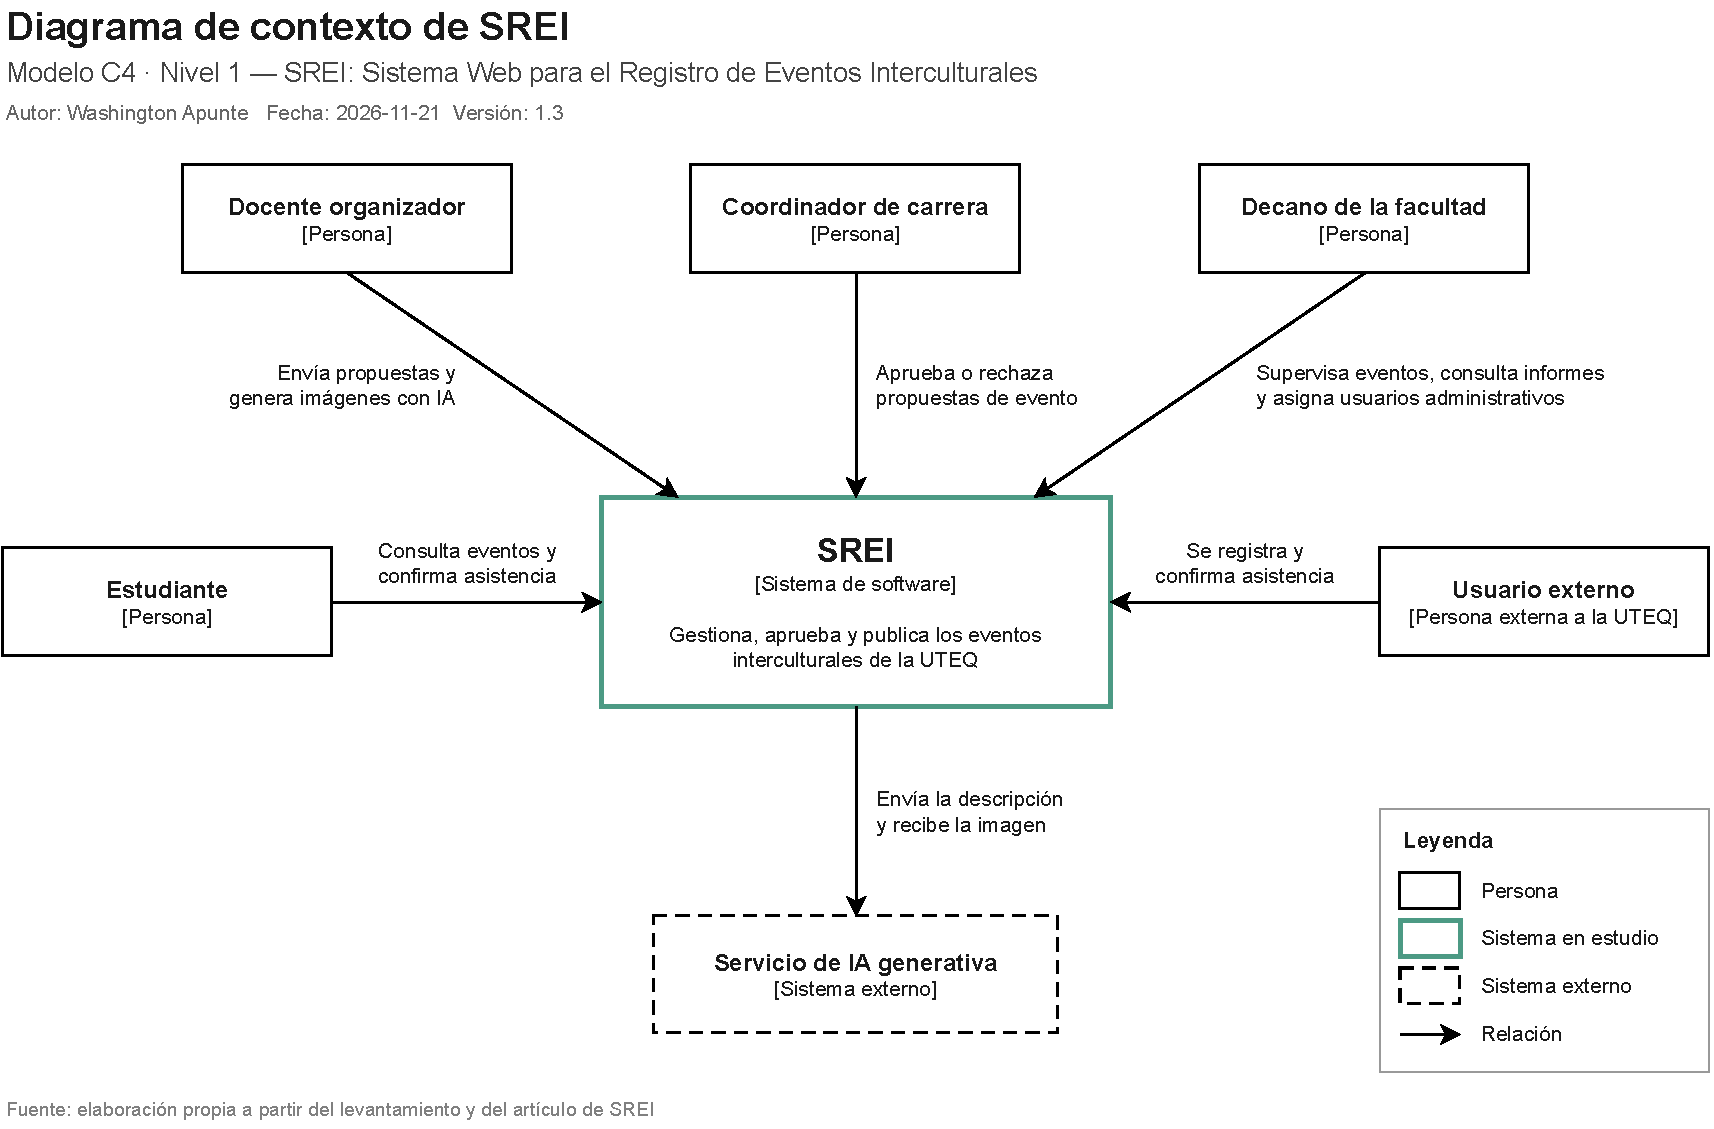
\includegraphics[width=\textwidth]{diagramas/c4-contexto.pdf}
  \caption{Diagrama de contexto (C4, nivel 1). Fuente: elaboración propia.}
  \label{fig:c4-contexto}
\end{figure}

\subsection{Contenedores}
La Figura~\ref{fig:c4-contenedores} muestra lo que hay dentro de SREI. 
Los usuarios entran por una aplicación web hecha en Angular 17, 
que se comunica con tres servicios Spring Boot: servicio-eventos en el puerto 8080, 
servicio-consulta en el puerto 8081 y servicio-usuarios. 
En el diseño, cada servicio guarda sus datos en su propia base PostgreSQL. 
Por ahora solo funcionan servicio-eventos y servicio-consulta, con el enlace INT-01, 
por el que servicio-consulta le pide los datos de un evento a servicio-eventos. 
La aplicación web, servicio-usuarios, las tres bases de datos y los demás enlaces todavía están previstos,
por eso se dibujan con línea punteada. 
El servicio de IA queda fuera de la frontera del sistema y se conectará desde servicio-eventos.

\begin{figure}[p]
  \centering
  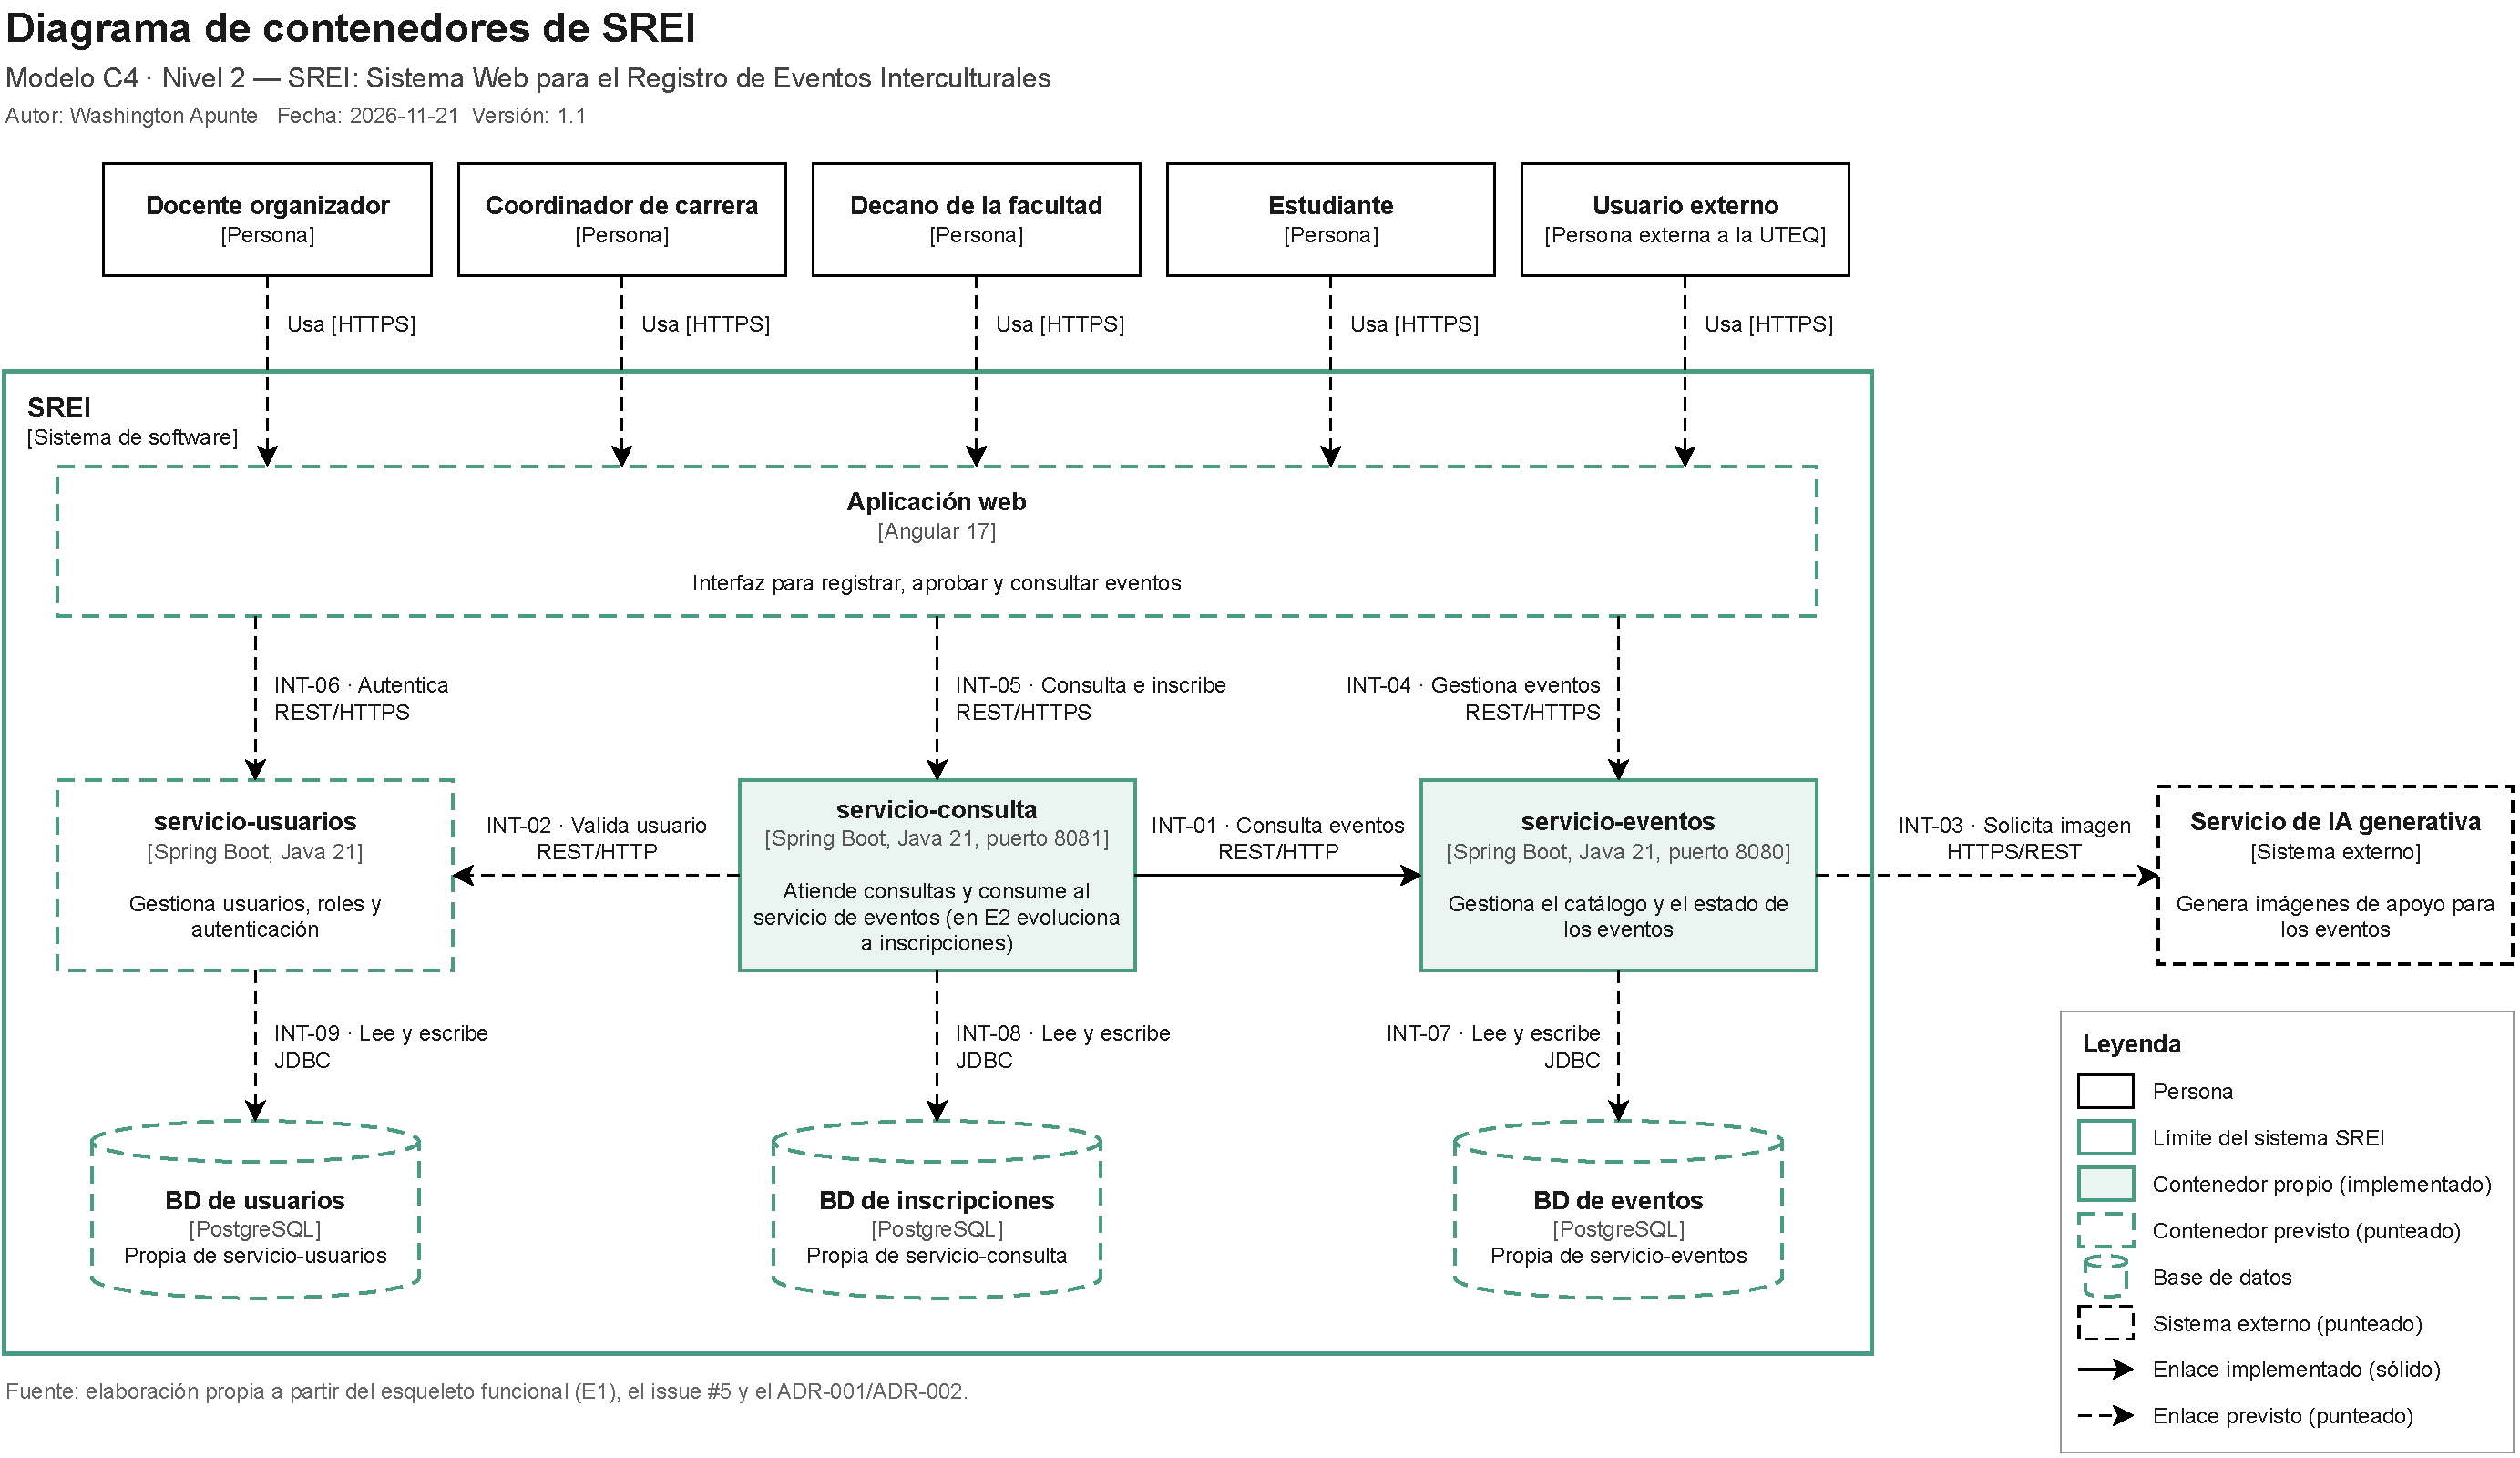
\includegraphics[width=0.9\textheight, height=0.85\textwidth, keepaspectratio, angle=90]{diagramas/c4-contenedores.pdf}
  \caption{Diagrama de contenedores (C4, nivel 2). Fuente: elaboración propia.}
  \label{fig:c4-contenedores}
\end{figure}

\subsection{Por qué un sistema distribuido y no un monolito}
Hoy SREI es un monolito: un solo backend y una sola base de datos hacen todo el trabajo. 
El problema es que una parte lenta frena a las demás. Puede pasar, por ejemplo, con la generación de imágenes, 
que depende de un servicio de IA que no controlamos. Mientras la IA no responde, 
cada petición sigue ocupando un hilo del mismo servidor que atiende el inicio de sesión y las inscripciones. 
Cuando esas esperas se acumulan, el servidor ya no tiene hilos para atender a nadie más y todo SREI se vuelve lento. 
Además, el PFC exige un sistema distribuido, y un monolito no lo es.

Con tres servicios, cada uno corre por separado y es dueño de su base de datos. 
La llamada a la IA saldrá solo de servicio-eventos (INT-03, previsto), así que si la IA se pone lenta, 
el problema se queda en ese servicio. El inicio de sesión, que maneja servicio-usuarios, sigue funcionando, 
y servicio-consulta solo se ve afectado cuando necesita datos de eventos. Separar los datos también ayuda. 
Como ningún servicio lee la base de otro, un cambio en las tablas de eventos no obliga a tocar las de inscripciones o usuarios.

Esta decisión tiene costos que aceptamos. Hay más piezas que levantar y configurar, 
cada una con su puerto y su base. Ya no se pueden unir datos de distintos servicios con un JOIN, 
así que hay que pedirlos por la API. Y como los servicios se llaman de forma síncrona, si servicio-eventos se cae, 
servicio-consulta no puede completar la consulta y el usuario ve un error.

Las opciones consideradas y la decisión completa están en el ADR-001.

\section{Plan del proyecto y aportes}

\subsection{Organización del equipo}

El desarrollo del Sistema de Registro de Eventos Interculturales (SREI) se organiza mediante el marco de trabajo Scrum. El equipo distribuye sus responsabilidades de acuerdo con las actividades necesarias para el levantamiento de requisitos, el diseño de la solución, el desarrollo y la documentación del sistema.

La organización busca que cada integrante tenga actividades definidas y que los avances puedan revisarse mediante las evidencias registradas en el repositorio del proyecto.

\subsection{Roles y responsabilidades}

\begin{longtable}{p{0.28\textwidth} p{0.22\textwidth} p{0.40\textwidth}}
\caption{Participantes y responsabilidades del proyecto}\\
\toprule
\textbf{Integrante} & \textbf{Rol} & \textbf{Responsabilidad}\\
\midrule
\endfirsthead

\toprule
\textbf{Integrante} & \textbf{Rol} & \textbf{Responsabilidad}\\
\midrule
\endhead

Dr. Gleiston Cicerón Guerrero Ulloa &
Scrum Master &
Facilitador externo y tutor académico del proceso Scrum.\\

Washington Germán Apunte Pazmiño &
Integrante del equipo &
Arquitectura y documentación de calidad del sistema.\\

Jordan Josue Loor Suárez &
Integrante del equipo &
Levantamiento de requisitos, documentación y seguimiento de los aportes.\\

Steffanny del Rocío Loor Suárez &
Integrante del equipo &
Desarrollo del esqueleto del sistema y comunicación entre servicios.\\

\bottomrule
\end{longtable}

Los Product Owners que proporcionan requisitos y orientaciones para el sistema son:

\begin{itemize}
    \item Ing. Jéssica Alexandra Ponce Ordoñez, coordinadora de la carrera de Software.
    \item Ing. Washington Alberto Chiriboga Casanova, decano de la Facultad de Ciencias de la Computación y Diseño Digital.
    \item Msc. Elizabeth Johanna Contreras Jara, docente de Educación Inicial de la Facultad de Ciencias de la Educación.
\end{itemize}

\subsection{Organización del trabajo}

Para facilitar el desarrollo, las actividades se distribuyen en bloques de trabajo relacionados con los entregables del proyecto:

\subsubsection{Asignación de roles técnicos}

La distribución de responsabilidades técnicas se establece de acuerdo con las actividades asignadas a los tres integrantes del equipo. Debido a que se requieren cuatro responsabilidades, uno de los integrantes asume dos roles.

\begin{longtable}{p{0.32\textwidth} p{0.28\textwidth} p{0.30\textwidth}}
\caption{Asignación de roles técnicos}\\
\toprule
\textbf{Integrante} & \textbf{Rol} & \textbf{Responsabilidad}\\
\midrule
\endfirsthead

\toprule
\textbf{Integrante} & \textbf{Rol} & \textbf{Responsabilidad}\\
\midrule
\endhead

Washington Germán Apunte Pazmiño &
Arquitecto &
Diseño de la arquitectura y documentación de sus componentes.\\

Washington Germán Apunte Pazmiño &
Responsable de Calidad &
Seguimiento de los criterios de calidad y verificación de los requisitos.\\

Jordan Josue Loor Suárez &
Responsable de Requisitos y Documentación &
Levantamiento, organización y documentación de los requisitos del sistema.\\

Steffanny del Rocío Loor Suárez &
Líder de Desarrollo &
Implementación del esqueleto del sistema, desarrollo de servicios y comprobación de la comunicación entre componentes.\\

\bottomrule
\end{longtable}

\subsection{Cronograma de entregas}

El proyecto se organiza en cuatro entregas principales, distribuidas de acuerdo con las semanas establecidas en el encuadre de la asignatura.

\begin{longtable}{p{0.14\textwidth} p{0.15\textwidth} p{0.58\textwidth}}
\caption{Planificación general de las entregas}\\
\toprule
\textbf{Entrega} & \textbf{Semana} & \textbf{Actividades principales}\\
\midrule
\endfirsthead

\toprule
\textbf{Entrega} & \textbf{Semana} & \textbf{Actividades principales}\\
\midrule
\endhead

E1 & 5 &
Definición del proyecto, levantamiento y especificación de requisitos y arquitectura inicial.\\

E2 & 9 &
Desarrollo de microservicios, definición de API e implementación de contenedores.\\

E3 & 13 &
Integración de la base de datos distribuida y procesamiento de información.\\

E4 & 17 &
Integración final del sistema, evaluación de calidad, pruebas y defensa del proyecto.\\

\bottomrule
\end{longtable}

Las actividades específicas y sus fechas de ejecución se gestionan de acuerdo con la planificación y los acuerdos establecidos por el equipo.

\subsection{Control de versiones y colaboración}

El repositorio de GitHub se utiliza para mantener el historial de cambios y facilitar la colaboración entre los integrantes. Cada estudiante trabaja en una rama propia y registra sus avances mediante commits que describen el trabajo realizado.

Los cambios se incorporan a la rama principal mediante solicitudes de integración (Pull Requests), en las que se revisa que los archivos correspondan al bloque de trabajo desarrollado.

Para evitar incorporar archivos temporales o cambios incompletos, se agregan explícitamente los archivos que forman parte de cada avance. Antes de realizar un commit se revisan los cambios preparados y se comprueba que no existan errores de formato.

El seguimiento de las actividades se complementa mediante los issues y el tablero de GitHub Projects, donde se pueden organizar las tareas, identificar a sus responsables y consultar su estado de avance.

\subsection{Seguimiento y evidencias}

El seguimiento de las actividades se realiza mediante los issues, commits y Pull Requests del repositorio. Estos elementos permiten identificar qué actividad se desarrolló, quién la realizó y qué archivos fueron modificados.

Las evidencias de diseño, levantamiento y ejecución se organizan en las carpetas correspondientes del repositorio:

\begin{itemize}
    \item \texttt{evidencias/levantamiento/}: documentos y registros relacionados con la recopilación de información.
    \item \texttt{evidencias/levantamiento/entrevistas/}: grabaciones de entrevistas y validaciones realizadas con los interesados.
    \item \texttt{evidencias/diseno/}: evidencias de diagramas y decisiones de diseño.
    \item \texttt{evidencias/ejecucion/}: capturas y resultados de las comprobaciones realizadas.
\end{itemize}

Los issues y el tablero de seguimiento permiten relacionar las actividades planificadas con los avances realizados. Los enlaces específicos se incorporarán en el registro de evidencias del proyecto.

\subsection{Registro de aportes individuales}

La siguiente tabla presenta los aportes identificados en el historial disponible del repositorio. Los identificadores de commit permiten localizar los cambios y revisar los archivos incorporados.

\begin{longtable}{p{0.20\textwidth} p{0.47\textwidth} p{0.23\textwidth}}
\caption{Registro de aportes individuales}\\
\toprule
\textbf{Integrante} & \textbf{Aporte registrado} & \textbf{Evidencia}\\
\midrule
\endfirsthead

\toprule
\textbf{Integrante} & \textbf{Aporte registrado} & \textbf{Evidencia}\\
\midrule
\endhead

Jordan Loor Suárez &
Documentación del contexto y antecedentes del proyecto SREI. &
Commit 089990a.\\

Jordan Loor Suárez &
Elaboración de historias de usuario, criterios de aceptación y requisitos del sistema. &
Commit 329f5cc.\\

Jordan Loor Suárez &
Organización de roles, responsabilidades, cronograma y registro de aportes. &
Commit 111a8b5.\\

Washington Apunte Pazmiño &
Elaboración de la arquitectura, documentación de requisitos no funcionales y análisis CAP/PACELC. &
Commits 5ee9e54, 08e6324 y 4563e78.\\

Steffanny del Rocío Loor Suárez &
Implementación del servicio proveedor de eventos, desarrollo del consumidor REST y documentación de la comunicación entre servicios. &
Commits 452b5c9, 4e11ee2 y f656a31.\\

\bottomrule
\end{longtable}

El registro presenta los aportes identificados en el historial del repositorio. Los identificadores de commit permiten consultar los cambios realizados y relacionarlos con las actividades asignadas a cada integrante. La tabla podrá ampliarse conforme se incorporen nuevos avances al proyecto.

\subsection{Uso de herramientas de inteligencia artificial}

Se utilizaron herramientas de inteligencia artificial como apoyo durante la elaboración y organización de la documentación del proyecto. Estas herramientas facilitaron la revisión de la redacción, la organización de información y la comprensión de algunos aspectos técnicos.

El contenido generado o sugerido mediante estas herramientas debe ser revisado por los integrantes antes de incorporarse a los entregables. La información, los requisitos, las decisiones técnicas y las evidencias presentadas deben corresponder al trabajo realizado y a las fuentes consultadas.

La utilización de estas herramientas no sustituye la revisión del equipo ni la responsabilidad de sus integrantes sobre el contenido final.


\newpage
\printbibliography[title={Referencias bibliográficas}]

\end{document}
